\documentclass[11pt,a4paper,spanish]{book}
\usepackage{estilo_unir-1}
\hypersetup{
	colorlinks   = true, %Colours links instead of ugly boxes
	urlcolor     = blue, %Colour for external hyperlinks
	linkcolor    = black, %Colour of internal links
	citecolor   = red %Colour of citations
}
\usepackage[nottoc]{tocbibind}

%---------------------------
%título de la asignatura, trabajo y autor
%---------------------------
\subject{Nombre de la asignatura}
\title{Escribir el título del documento}
\author{Nombre y Apellidos de los autores}
\profesor{Nombre del profesor}
\date{introducir fecha}

%---------------------------
%marges
%---------------------------
%\usepackage[margin=1.9cm]{geometry}
%---------------------------
%---------------------------
%---------------------------
%---------------------------
\begin{document}
\renewcommand{\listfigurename}{Índice de figuras}
\renewcommand{\listtablename}{Índice de tablas}
\renewcommand{\contentsname}{Índice de contenidos}
\renewcommand{\figurename}{Figura}
\renewcommand{\tablename}{Tabla} 

\maketitle
\frontmatter
\tableofcontents
\listoffigures
Fijaos que SOLO aparece el título de cada figura, no aparece toda la leyenda ni la fuente. \\
(QUITAR ESTA PÁGINA SI NO HAY FIGURAS) 
\listoftables
Fijaos que SOLO aparece el título de cada tabla, no aparece toda la leyenda ni la fuente. \\
(QUITAR ESTA PÁGINA SI NO HAY TABLAS)

\chapter{Resumen}
En esta Sección se introducirá un breve resumen en español del trabajo realizado (extensión máxima: esta página). 
\newline

Este resumen debe incluir el propósito de la investigación, la metodología, los resultados y las conclusiones (obviamente, todo muy resumido, pero así se sabe de un vistazo lo que se va uno a encontrar a continuación). 
\newline

En general, los conceptos deben estar claramente explicados (de forma resumida, repito) para que el propio resumen sea autoconsistente.

\vspace{0.5cm}
{\bf Palabras clave:} se deben incluir de 4 a 6 conceptos clave en español, significativos para el contenido del Trabajo (pueden ser conceptos formados por más de una palabra, pero DEBEN ser significativos). Por favor no incluir siglas, y todas las palabras en minúsculas

\chapter{Abstract}
This Section should include the english version of the previous Resumen.

\vspace{0.5cm}
{\bf Keywords:} please include between 4 to 6 key concepts in english, relevant to the content of this report (each concept might include multiple words). Please, do not include acronims and all words should be lower letters.

\mainmatter

\chapter{Introducción}

En la Introducción se debe resumir de forma esquemática pero suficientemente clara lo esencial de cada una de las partes del trabajo y, sobre todo, aprovechar para explicar conceptos que puedan ser de utilidad después. 
\newline

La lectura de esta parte debe contextualizar perfectamente todo el Trabajo y debe estar PLAGADA DE REFERENCIAS (más adelante se describe cómo hacerlo).
\newline

Es una parte muy importante de la memoria. Las ideas principales a transmitir son la identificación del problema a tratar, la justificación de su importancia, esbozo de los objetivos generales a grandes rasgos y un adelanto de la contribución que esperas hacer.

A modo de guía, la Introducción debe contener estos tres apartados:
\begin{itemize}
\item Motivación / justificación del tema a tratar
\item Planteamiento del Trabajo (atención a la mayúscula de "Trabajo": cuando nos referimos a nuestro documento, ese Trabajo va en mayúscula)
\item Estructura del Trabajo
\end{itemize}

\vspace{1cm}
{\bf{ATENCIÓN, CÓMO REFERENCIAR.}}

A continuación vamos a ver qué son, qué no son y para qué  sirven las referencias bibliográficas:
\begin{itemize}
	\item las referencias NO están para rellenar
	\item las referencias SÍ son un TRIBUTO a las personas que hicieron en primer lugar una investigación o aportaron una idea
	\item la referencias citan trabajo que acompaña una idea o un concepto, NO se usa UNA referencia para todo un párrafo que aglutina diferentes conceptos
	\item deben citarse LOS TRABAJOS ORIGINALES DE LOS AUTORES, y no un libro de texto donde he visto que hablan de algo
	\item os libros de texto se pueden referencial excepcionalmente, porque el libro es sobresaliente y conocido en el campo y/o porque quiero apoyarme en una explicación conocida para un determinado concepto o cuestión, pero no como origen del concepto del que se habla
\end{itemize}

\vspace{1cm}
{\bf{VEAMOS EJEMPLOS DE CITAS.}}

Vamos a ver los dos tipos de citas que vamos a utilizar normalmente en los trabajos y actividades:
\begin{itemize}
	\item CITA INDIRECTA: estamos hablando de algo e introcimos la referencia sobre la que apoyamos esa idea. Por ejemplo, hablado de los procesadores de texto, LATEX  \citep{lamport1994} es tipo de editor con el que se consiguen resultados de gran calidad
	\item CITA DIRECTA: nos referimos directamente a un trabajo y lo citamos. Por ejemplo, según \cite{ackerman2017}, la liga de fútbol inglesa debe tener torneos de desempate
\end{itemize}
\newline

Según el párrafo anterior con la cita indirecta aparecerá entre paréntesis el apellido y el año, separados por una coma; en el caso de varios autores, podrán aparecer hasta tres apellidos y, cuando son más, aparecerá el primero seguido de "et al." (y después el año separado con una coma). Con la cita directa solo va entre paréntesis el año, pero no los autores. Podéis mirar el apartado de Bibliografía para ver cómo han quedado estas citas.
\newline

En esta Actividad, cuando vamos a resolver problemas, PUEDE utilizarse libros de texto como referencias de procedimientos matemáticos que vamos a utilizar, pero sin olvidar el párrafo anterior. Es decir, sería conveniente citar ARTÍCULOS ORIGINALES de donde surgieron esos desarrollos.
\newline

Para consultar detenidamente la formas de referenciar, debéis seguir el formato APA del siguiente documento: \url{https://bibliografiaycitas.unir.net/documentos/APA_7ed_UNIR.pdf}


\chapter{Objetivos}

Esquematizar claramente los objetivos del trabajo, las ideas que queremos demostrar. Podemos tener varios tipos de objetivos. Por ejemplo, podemos tener un número de objetivos generales y otro de objetivos específicos. Deben ordenarse claramente.

\section{Objetivos generales}
Aquí vamos a exponer los objetivos generales. Es una forma de dar perspectiva al Trabajo. Debemos ser ambiciosos en esta exposición

\section{Objetivos específicos}
En esta Sección vamos a dar detalles concretos de lo que queremos conseguir. Por tanto, estos objetivos van al detalle.


\chapter{Enunciado del problema}

Esquematizar claramente los enunciados de los problemas, cuestiones o las ideas que queremos demostrar. Podemos extender el enunciado de la Actividad para mejorarlo o para dejar más claro aquello que vamos a solucionar.

\chapter{Desarrollo del Trabajo}

Aquí desarrollaremos nuestro trabajo. Contrastaremos la ideas entre varios autores y, si es posible, con las nuestras. Podemos incluir las secciones y subsecciones que necesitemos.
\newline

Tanto en esta Sección, como en el resto del Trabajo, se debe cuidar la redacción, el uso de las comas, puntos, puntos y coma, puntos y aparte y demás recursos. Fijaos en esta plantilla como estan escritas ciertas palabras que usamos mucho: \emph{Sección xx}, pero \emph{secciones}; \emph{Figura xx}, pero \emph{figuras}; \emph{Ecuación xx}, pero \emph{ecuaciones}; etc... Podéis echar un vistazo a trabajos de fin de estudios para comprobar la organización, ortografía y redacción de un trabajo a este nivel. En el repositorio de UNIR tenéis la posibilidad de acceder a trabajos presentados como TFMs en esta Titulación que os servirán de modelo: \url{https://reunir.unir.net/handle/123456789/6218}
\newline

Las figuras y tablas tienen que tener su numeración y su título. Además, se debe indicar la fuente, si es de elaboración propia o se ha tomado de alguna referencia.
\newline

Por ejemplo:

\begin{figure}[h]
	\centerline{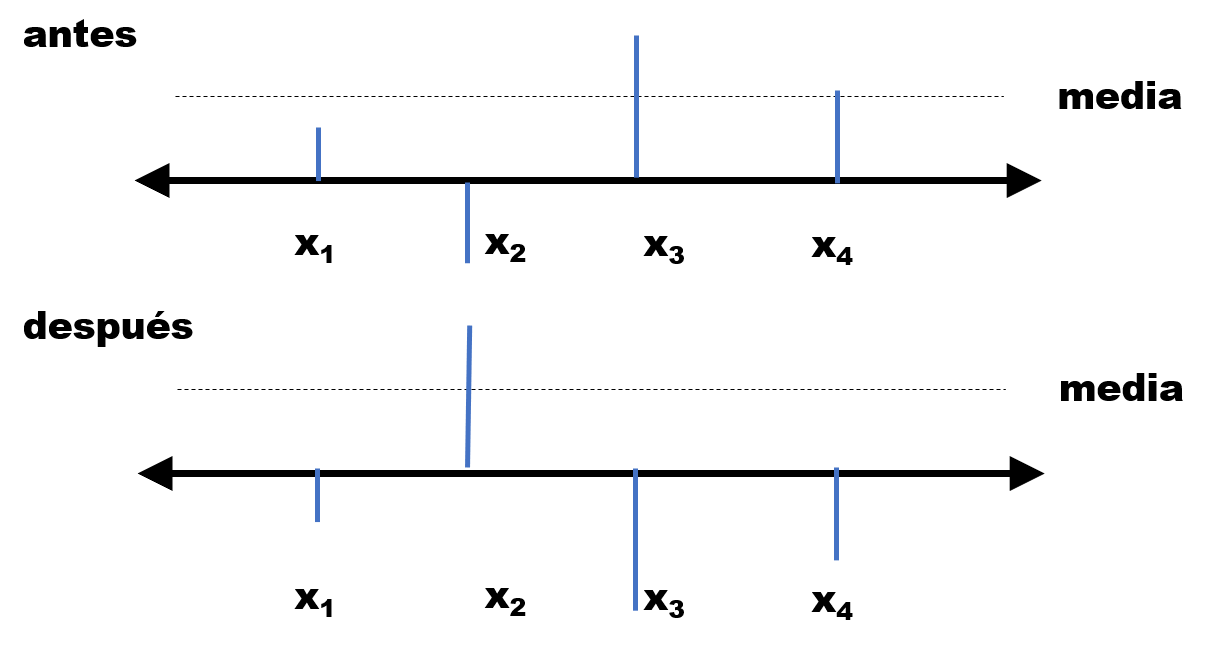
\includegraphics[scale=0.4]{figuras/inversionmedia.png}}
	\caption[Inversión sobre la media del algoritmo de Grover]{Inversión sobre la media del algoritmo de Grover. El conjunto de ${x_i}$ son las amplitudes de cada estado cuántico. La línea discontinua es la media de las amplitudes. Después de cada inversión, la amplitudes grandes se vuelven más grandes y las pequeñas más pequeñas. Fuente: elaboración propia}
	\label{fig:inversionmedia}
\end{figure}

En la Figura~\ref{fig:inversionmedia} vemos que es una figura de elaboración propia, mientras que la Figura~\ref{fig:distprob}, la fuente es un artículo cuya referencia viene indicada y el artículo es incluído en la Bibliografía.
\newline
\begin{figure}[h]
	\centerline{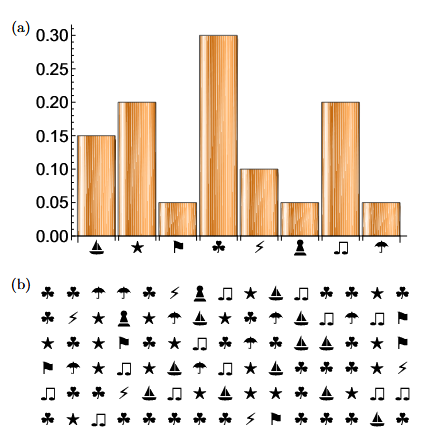
\includegraphics[scale=0.6]{figuras/distribucionprobabilidades.png}}
	\caption[Distribución de probabilidades]{a) Un ejemplo de distribución de probabilidad sobre 8 símbolos. (b) 100 muestras aleatorias de la distribución de probabilidad.
		probabilidad. El objetivo de un problema de muestreo es calcular muestras como las secuencias mostradas en (b) cuya complejidad	puede ser diferente a la complejidad de calcular la distribución de probabilidad (a). Fuente: \cite{lund2017}}
	\label{fig:distprob}
\end{figure}

Se incluye la Tabla~\ref{tab:balance} a modo de ejemplo. Solo contiene información sobre el balance de dos empresas ficticias. Debe incluirse también una leyenda, debajo de la tabla, junto con la fuente.
\newline
\begin{table}[Ht]
	\centering % esto centra la tabla
	\begin{tabular}{c c c c} % centra las 4 columnas
		\hline\hline %incluye líneas horizontales dobles
		Empresa & Ingresos & Gastos & Otros \\ [0.5ex] 
		\hline 
		Tintileo  & 50000 & 83700 & 97000 \\
		Packandgo & 47000 & 87700 & 23000 \\
		\hline
	\end{tabular}
	\caption[Balance de empresas]{Dos empresas ficticias con las columnas de ingresos y gastos, para dos años que no se especifican. Fuente: elaboración propia.}
	\label{tab:balance}
	\label{table:nonlin} % is used to refer this table in the text
\end{table}


\chapter{Conclusiones}

Las conclusiones es otra parte muy IMPORTANTE de la memoria. Deben ser muy claras. Si es posible se pueden itemizar o, mejor, poner un párrafo por idea con un pequeño título ilustrativo. En cualquier caso debe incluir los logros conseguidos y la importancia de los mismos, siempre desde un punto de vista crítico y resaltando las partes importantes.

\vspace{1cm}
{\bf{SOBRE LA EXTENSIÓN DEL TRABAJO}}
\newline

El Trabajo debe tener una extensión de $\sim$10 páginas. Los trabajos que se alejen de forma significativa de esta condición NO SE ACEPTARÁN. Las páginas que cuentan son las que van de la Introducción hasta estas Conclusiones. NO CUENTAN aquellas dedicadas a apéndices o a la Bibliografía.


\begin{thebibliography}{99}
\bibitem[Lamport(1994)]{lamport1994} Lamport, L. (1994) \emph{\LaTeX: a document preparation system}, Addison
Wesley, Massachusetts, 2nd ed.
\bibitem[Ackerman(2017)]{ackerman2017} Ackerman, E. (2017) Why the English Premier League Should Have Playoffs.  McGraw Hill. London. 
\bibitem[Lund(2017)]{lund2017} Lund, A. P. and Bremner, Michael J. and Ralph, T. C. (2017) Quantum sampling problems, BosonSampling and quantum supremacy, npj Quantum Information 3: 15
\end{thebibliography}

\vspace{2cm}
Aún a riesgo de ser redundante, repito aquí que para consultar detenidamente la formas de referenciar, debéis seguir el formato APA del siguiente documento: \url{https://bibliografiaycitas.unir.net/documentos/APA_7ed_UNIR.pdf}

%\bibliographystyle{plain} 
%\bibliography{bibliografia}

\end{document}





















